\documentclass[letterpaper, 12pt]{article}
\usepackage[top=2cm,bottom=1cm,left=0.75in,right=0.75in,headheight=17pt, % as per the warning by fancyhdr
includehead,includefoot,
heightrounded, % to avoid spurious underfull messages
]{geometry}
\addtolength{\topmargin}{-.25in}
\usepackage{fancyhdr}
\pagestyle{fancy}
\usepackage{graphicx}
\usepackage{lastpage}
\usepackage{gensymb}
\usepackage[american]{circuitikz}

\begin{document}
\fancyhead[l]{	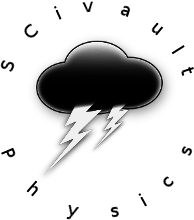
\includegraphics[height=1.2cm]{../Logo/sp.png} Name:}
\fancyhead[r]{REFERENCE MATERIAL}
\cfoot{\thepage\ of \pageref{LastPage}}
	


\begin{center}Things to Memorize: Circuits
\end{center}

\subsection*{Basics of Circuits}
\begin{itemize}
	\item For Electricity to flow, a circuit must make a complete path between the two sides of the source. 
	\begin{itemize}
		\item A Circuit that does not have a complete path is called an \textbf{Open Circuit}.  No current flows in an open circuit.
		\item A circuit that connects the two sides of the source without connecting any components in between is a \textbf{Short Circuit}.  Large currents flow in short circuits, which often lead to fires and other bad things.
	\end{itemize}
	\item \textbf{Voltage} is the energy per charge.
	\item \textbf{Current} is the amount of charge that passes a point in one second. 
	\item \textbf{Resistance} is the hindrance to the flow of charge.
\end{itemize}
\subsection*{Circuit Components}
\begin{center}
	\begin{tabular}{|c | p{1in} | p{3.5in}  |}

		\hline
		
		Battery &  
			
			\begin{circuitikz}
					
			\draw (0,0) to[battery=$B_1$] (2,0);
			\end{circuitikz}
	   	&  \textit{Source} - Stores energy for a circuit chemically. \\ \hline
		
		Resistor & 
		
			\begin{circuitikz}
				\vspace{1in}
			\draw (0,0) to[R=$R_1$] (2,0);
			\end{circuitikz} 
	  	&  \vspace{-.25in} Dissipates electrical energy as heat; resists the flow of current.    \\ \hline
	  	
	 Light Bulb & \vspace{0.5in} & Similar to a resistor, but resistance changes with temperature. \\ \hline
		Light Emitting Diode (LED) &  
		\begin{circuitikz}
			
			\draw (0,0) to[leDo=$LED_1$] (2,0);
		\end{circuitikz}
		 & Turns electrical enegy into light; only lets current flow one way.  Must be used in series with a resistor or will be destroyed.  \\ \hline
		 
		Capacitor &  
		\begin{circuitikz}
			
			\draw (0,0) to[C=$C_1$] (2,0);
		\end{circuitikz}
		 & Stores energy in an electrical field.   \\ \hline
		Inductor &
			\begin{circuitikz}
			
			\draw (0,0) to[L=$L_1$] (2,0);
		\end{circuitikz}
		  & Stores energy in a magnetic field. \\ \hline
		Ammeter & 
		\begin{circuitikz}
			\draw (0,0) to[ammeter] (2,0);
		\end{circuitikz}
		 & Measures Current \\ \hline 
		Voltmeter &
		\begin{circuitikz}
			\draw (0,0) to[voltmeter] (2,0);
		\end{circuitikz}
		 & Measures Voltage \\ \hline		
	\end{tabular}
\end{center}
	\vspace{1in}
	
\subsection*{Resistors}
\begin{itemize}
	\item Resistors are measured in Ohms ($\Omega$). 
	\item Resistors follow ohm's law.
	\item Resistors are usually made of carbon, silicon, or metal oxides.  
	\item The resistance of a resistor can be calculated using its dimensions and the resistivity of the material it is made of.
	
\end{itemize}

\subsection*{Capacitors}
\begin{itemize}
	\item Capacitors are measured in Farads (F).
	\item Capacitors are really just two sheets of metal separated by a very small gap of air, vacuum, or some other nonconducting material.
	\item The capacitance of any capacitor can be calculated from its dimensions and the dielectric constant of any material between the two plates.
	
\end{itemize}

\subsection*{Inductors}
\begin{itemize}
	\item Inductors are measured in Henries (H).
	\item Inductors are really just a coil of wire.  
	\item Calculating inductance is non-trivial.  Most inductors are measured experimentally.	
\end{itemize}



\subsection*{Types of Circuits}
	\begin{itemize}
		\item \textbf{Series circuits} have only one path for current to flow.
			\begin{itemize}
				\item Resistors in Series \textbf{add}.
				\item Capacitors in Series \textbf{add as reciprocals}.
				\item Current in series is \textbf{the same}.
				\item Voltage in series \textbf{adds up} to the voltage of the source. 
			\end{itemize}
		\item \textbf{Parallel Circuits} have multiple paths for current to flow. 
			\begin{itemize}
				\item Resistors in Parallel \textbf{add as reciprocals}.
				\item Capacitors in Parallel \textbf{add.}
				\item Current in Parallel \textbf{adds up} to the current provided by the source.
				\item Voltages in Parallel are \textbf{the same}.
			\end{itemize}
		\item Some circuits have parts that are in series and other parts that are in parallel.
	\end{itemize}
\subsection*{Meters and Measurements}
\begin{itemize}
	\item Ammeters should be connected in \textbf{Series}.
	\item Voltmeters should be connected in \textbf{Parallel}.
\end{itemize}

\subsection*{Kirchhoff's Laws}
\begin{itemize}
	\item \textbf{Kirchhoff's Current Law} states that the sum of the currents flowing into a junction must equal the sum of the currents flowing out of a junction. 
	\begin{itemize}
		\item Also known as Kirchhoff's First Law, Kirchhoff's Point rule, Kirchhoff's Junction Rule, and Kirchhoff's Nodal Rule.
	\end{itemize}
	\item \textbf{Kirchhoff's Voltage Law} states that the sum of the voltage drops around any closed loop must equal zero.
	\begin{itemize}
		\item This implies in a circuit with a single source, the total voltage of all sinks is equal to the voltage of the source.
		\item Also known as Kirchhoff's Second Law, Kirchhoff's Loop Rule, Kirchhoff's Mesh Rule, and Kirchhoff's Second Rule.
	\end{itemize}
	
\end{itemize}


\end{document}
